\chapter{Prezentarea proiectului}

Acest capitol al lucrării are ca scop prezentarea principalelor concepte tehnice și
arhitecturale care stau la baza implementării sistemului de compilare distribuită,
descrierea deciziilor de proiectare care modelează structura sistemului și a soluțiilor
practice propuse pentru etapa implementare. Sunt analizate în amănunt tehnologiile utilizate,
pentru a crea o imagine de ansamblu a modului în care acestea influențează arhitectura sistemului.

\section{Fundamentare teoretică}

\subsection{Sisteme distribuite}

% Împreună cu capitolul următor reprezintă cca. 70\% din lucrare. 

% Titlul acestui capitol nu este unul impus și nici nu corespunde neapărat unui singur capitol. 
% Titlul indică mai degrabă o parte (importantă și centrală, de altfel) a lucrării, în care se prezintă 
% ceea ce s-a realizat efectiv: contribuțiile autorului. Organizarea acestei părți este dependentă și 
% specifică fiecărei lucrări în parte și este stabilită de către fiecare autor după cum i se pare mai 
% potrivit pentru tema lui. Ea poate cuprinde prezentarea unor concepte teoretice (unelte sau tehnici
% matematice folosite în lucrare, prezentarea sau introducerea unor concepte teoretice etc.),  o 
% analiză a diferitelor metode/algoritmi/tehnologii etc. luate în considerare sau dezvoltate de către 
% autor, o prezentare a unui design (mai mult sau mai puțin detaliat) sau chiar detalii a unei 
% eventuale implementări/prototip, dacă e cazul.

% Trebuie remarcat însă faptul că această parte reprezintă contribuția personală a autorului, și în nici 
% un caz ea nu poate fi sinteza unor texte preluate din alte surse. Prin urmare, orice informații sunt 
% prezentate aici, ele trebuie să corespundă cel puțin unei interpretări/analize critice personale a 
% autorului, dacă nu chiar unor idei originale ale acestuia. 

Abordarea calculului distribuit presupune utilizarea resurselor provenite de la mai multe sisteme
de calcul interconectate pentru a contribui la rezolvarea sarcini, în mod colaborativ. Astfel, dificultatea
sarcinii nu rămâne rezervată unui singur sistem de calcul, ci este partiționată și distribuită în mod eficient
către mai multe sisteme, pe baza metodelor de balansare a sarcinii. Fiecare dintre nodurile participante își
pune la dispoziție atât capacitatea de calcul, precum și resursele de memorie, iar comunicarea cu celelalte
noduri participante, în scopul coordonării, se realizează de cele mai multe ori în cadrul unei rețele 
de calculatoare \cite{buyya1999high}.

Astfel, paradigma de calcul distribuit oferă avantaje semnificative, în ceea ce privește randamentul de procesare
a datelor și asigurarea desiponibilității serviciilor, către utilizatorii sistemului:

\begin{itemize}
    \item Toleranță la eșecuri - prin mecanisme de monitorizare periodică a stării de 
    disponibilitate a nodurilor din sistem, se pot remedia situațiile în care una dintre cererile
    ce trebuie soluționate nu poate fi deservită din cauza indisponibilității temporare a unui nod implicat,
    întrucât nodurile redundate ale sistemului pot prelua sarcina nefinalizată
    \item Folosirea eficientă a resurselor neutilizate - în general, un computer obișnuit poate să se afle în stare de 
    inactivitate cam în 70\% din timpul total de funcționare \cite{buyya1999high}, ceea ce înseamnă că aceste
    resurse computaționale nefolosite pot fi agregate eficient în cadrul unui sistem distribuit pentru a rezolva
    sarcini costisitoare, a căror realizare nu ar fi fezabilă folosind un singur sistem de calcul
    \item Balansarea volumului de lucru - în cazul în care un nod solitar din cadrul sistemului distribuit nu face 
    față volumului de lucru, alte noduri de calcul pot fi alocate în mod dinamic pentru a prelua
    din sarcini, fără a introduce ineficiențe legate de suprasaturarea resurselor unui anumit nod
    \item Scalabilitatea - limitările introduse de utilizarea unui singur sistem de calcul, al cărui potențial
    de performanță maximă este finit, pot fi mitigate prin introducerea de mai multe noduri participante, în funcție de
    nevoi 
    \item Distribuirea geografică convenabilă - întrucât nodurile participante ale sistemului comunică prin intermediul
    rețelelor de calculatoare, distribuirea nodurilor asupra unei arii geografice de mare întindere devine o posibilitate,
    iar pentru fiecare utilizator al sistemului se pot identifica resursele care sunt cel mai apropiate și implicit, cele
    mai facil de accesat, pentru a satisface solicitările
\end{itemize}

Pe de altă parte, implementarea paradigmei de calcul distribuit implică dezavantajul creșterii semnificative a gradului de
complexitate pentru realizarea unui sistem fiabil, din cauza necesității de a asigurara un mediu de comunicare stabil și performant,
dar și a garanției că sistemul are o stare globală consistentă. Pentru simplul fapt că informațiile
legate de starea sistemului sunt împărțite pe multiple noduri, există riscul să apară inconsistențe între informațiile reținute
de fiecare nod \cite{van2002distributed}.

De asemenea, idealul ca un sistem distribuit să se afle permanent într-o stare adecvată de funcționare se întemeiază pe asumpții
care nu sunt tot timpul adevărate:

\begin{itemize}
    \item Lățimea de bandă a canalelor de comunicație dintre noduri este infinită
    \item Structura rețelei și a nodurilor este omogenă
    \item Rețeaua este sigură
    \item Rețeaua este tot timpul dispponibilă
    \item Latența pentru transferurile de date dintre noduri este neglijabilă
\end{itemize}

În încheierea acestei secțiuni, oferim figura \ref{fig:distributed_sys}, pentru a ilustra structura generală a unui sistem 
distribuit, în care mai multe noduri comunică într-o rețea cu topologie \textbf{"bus"}.

\begin{figure}[H]
    \centering
    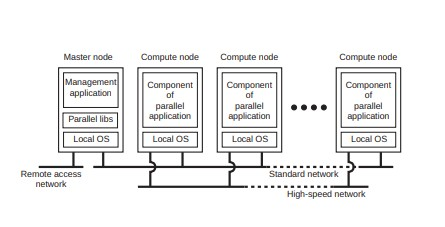
\includegraphics[width=0.8\linewidth, height=0.35\linewidth]{figures/distributed_system_bus.jpg}
    \caption{Sistem distribuit \cite{van2002distributed}}
    \label{fig:distributed_sys}
\end{figure}

\subsection{Mecanisme de concurență și paralelism}

Una dintre problemele pe care orice sistem distribuit trebuie să le rezolve o reprezintă asigurarea capacității
de comunicare simultană între un număr mare de noduri ale sistemului, pentru a oferi posibilitatea de scalare 
prin adăugarea de noduri suplimentare și a garanta că schimbul de informații dintre oricare două noduri nu 
trebuie să fie blocat până la finalizarea altor sarcini de calcul sau comunicare.

Având în vedere acest fapt, am ales să introduc în lucrare o secțiune ce prezintă fundamentele teoretice legate
de asigurarea concurenței, în contextul dezvoltării sistemelor distribuite.

Concurența constituie capacitatea unui sistem de a executa mai multe sarcini în mod simultan. Până la momentul
apariției sistemelor de calcul cu procesoare dotate cu mai multe nuclee, se crea impresia că mai multe sarcini
de procesare erau soluționate în paralel prin schimbarea frecventă a contextului de execuție pentru sarcinile
aflate în desfășurare \cite{reguera2025asynchronous}. În urma evoluției continue a resurselor hardware, au apărut 
mijloace multiple de asigurare a execuției concurente sau paralele.

Figura \ref{fig:conc_paral} are rolul de a ilustra diferența fundamentală dintre execuția concurentă și cea paralelă.

\begin{figure}[H]
    \centering
    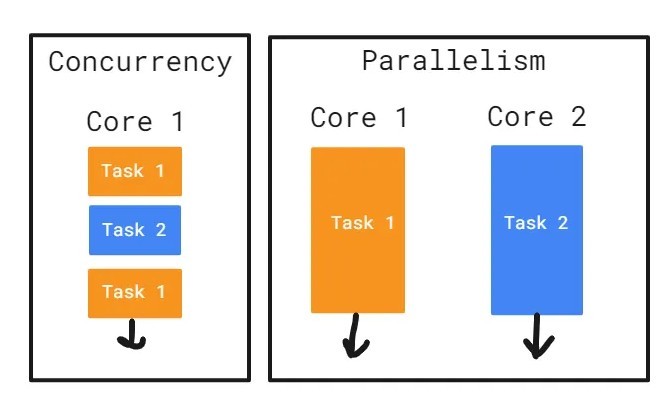
\includegraphics[width=0.8\linewidth, height=0.3\linewidth]{figures/concurrent_parallel.jpg}
    \caption{Concurență vs. paralelism \cite{Kizilarslan2024ParallelProgramming}}
    \label{fig:conc_paral}
\end{figure}

Așadar, concurența presupune ca sistemul să asigure evoluția mai multor sarcini independente, care sunt
active în același interval de timp și poate fi obținută prin comutare de context, fără a fi necesară utilizarea
unui procesor cu mai multe nuclee sau a mai multor sisteme de calcul. Spre exemplu, concurența task-urilor
este foarte utilă în momentul în care trebuie să așteptăm după un eveniment, fără a bloca execuția pentru restul
programului. Mai sugestiv, toate aplicațiile server actuale trebuie să rezolve problema \textbf{C10K} \cite{nenovasynchronous},
adică să asigure scalabilitatea aplicației pentru un număr mai mare de 10000 de conexiuni de rețea simultane, fără să epuizeze
resursele computaționale. De cele mai multe ori, asigurarea concurenței este suficientă pentru a nu bloca firul
principal de execuție al programului când se așteaptă finalizarea unei operațiuni \textbf{I/O} blocante 
("I/O-bound"\cite{reguera2025asynchronous}).

Pe de altă parte, paralelismul oferă posibilitatea de a executa, în același moment discret de timp, două sau mai
multe sarcini computaționale, fără a fi nevoie de executarea unei porțiuni din fiecare sarcină în mod secvențial
pentru o perioadă redusă de timp. Principalul caz de utilizare al execuției paralele îl constituie împărțirea volumului
de muncă între mai multe entități, cu scopul de a reduce durata de timp necesară pentru a finaliza procesarea 
("CPU-bound"\cite{reguera2025asynchronous}).

În secțiunile următoare vom explica funcționarea câtorva dintre mecanismele de concureță și paralelism utilizate pentru dezvoltarea
sistemului de compilare distribuită.

\subsubsection{Thread-uri}

Folosirea de multiple thread-uri\cite{williams2019c++} reprezintă o soluție eficientă pentru a rula mai multe task-uri în mod concurent, în
interiorul unui singur proces aflat în execuție. Una dintre diferențele principale dintre conceptul de thread și cel
de proces, o constituie faptul că în vreme ce un proces își gestionează spațiul de adrese de memorie și resurse în mod total
independent față de restul proceselor, mai multe thread-uri partajează aceleași resurse, ce aparțin procesului părinte.

Spre deosebire de procese, comunicarea între mai multe thread-uri active este mai facilă și mai eficientă, datorită 
spațiului de memorie partajat. De asemenea, împărțirea spațiului de memorie introduce necesitatea folosirii
unor mecanisme de sincronizare între firele de execuție (semafoare, excludere mutuală), pentru a împiedica coruperea datelor,
datorată manipulării simultane a resurselor partajate, de către mai multe thread-uri care rulează în paralel. 


